\documentclass{article}
\usepackage{amsmath,amssymb,graphicx}
\textwidth16cm
\textheight24cm
\oddsidemargin0em
\topmargin-1cm

\begin{document}
\begin{center}
\Large Tutorial on OCTOPUS
\end{center}

\vspace{1cm}

\begin{center}
\hspace*{-3cm}
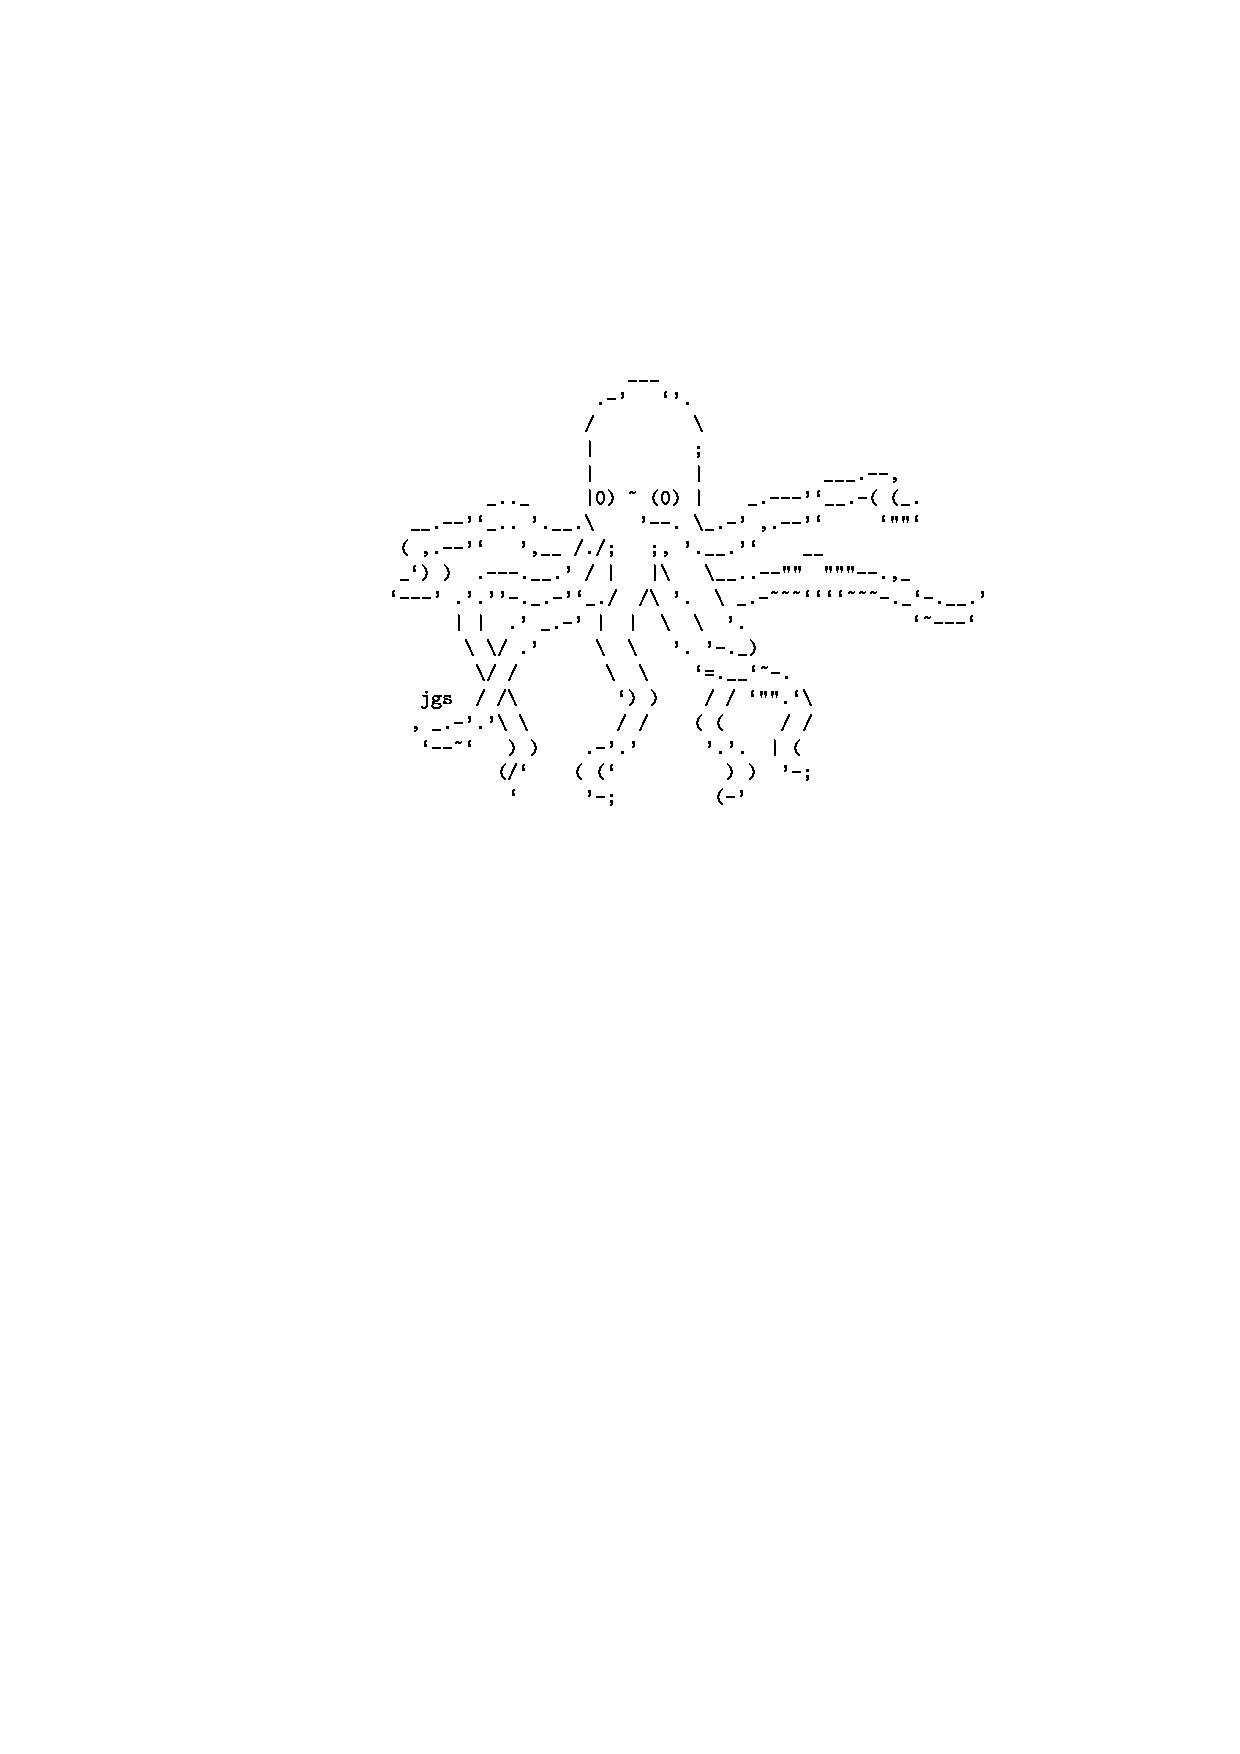
\includegraphics[height=5cm]{img/cover}
\end{center}

\begin{flushright}
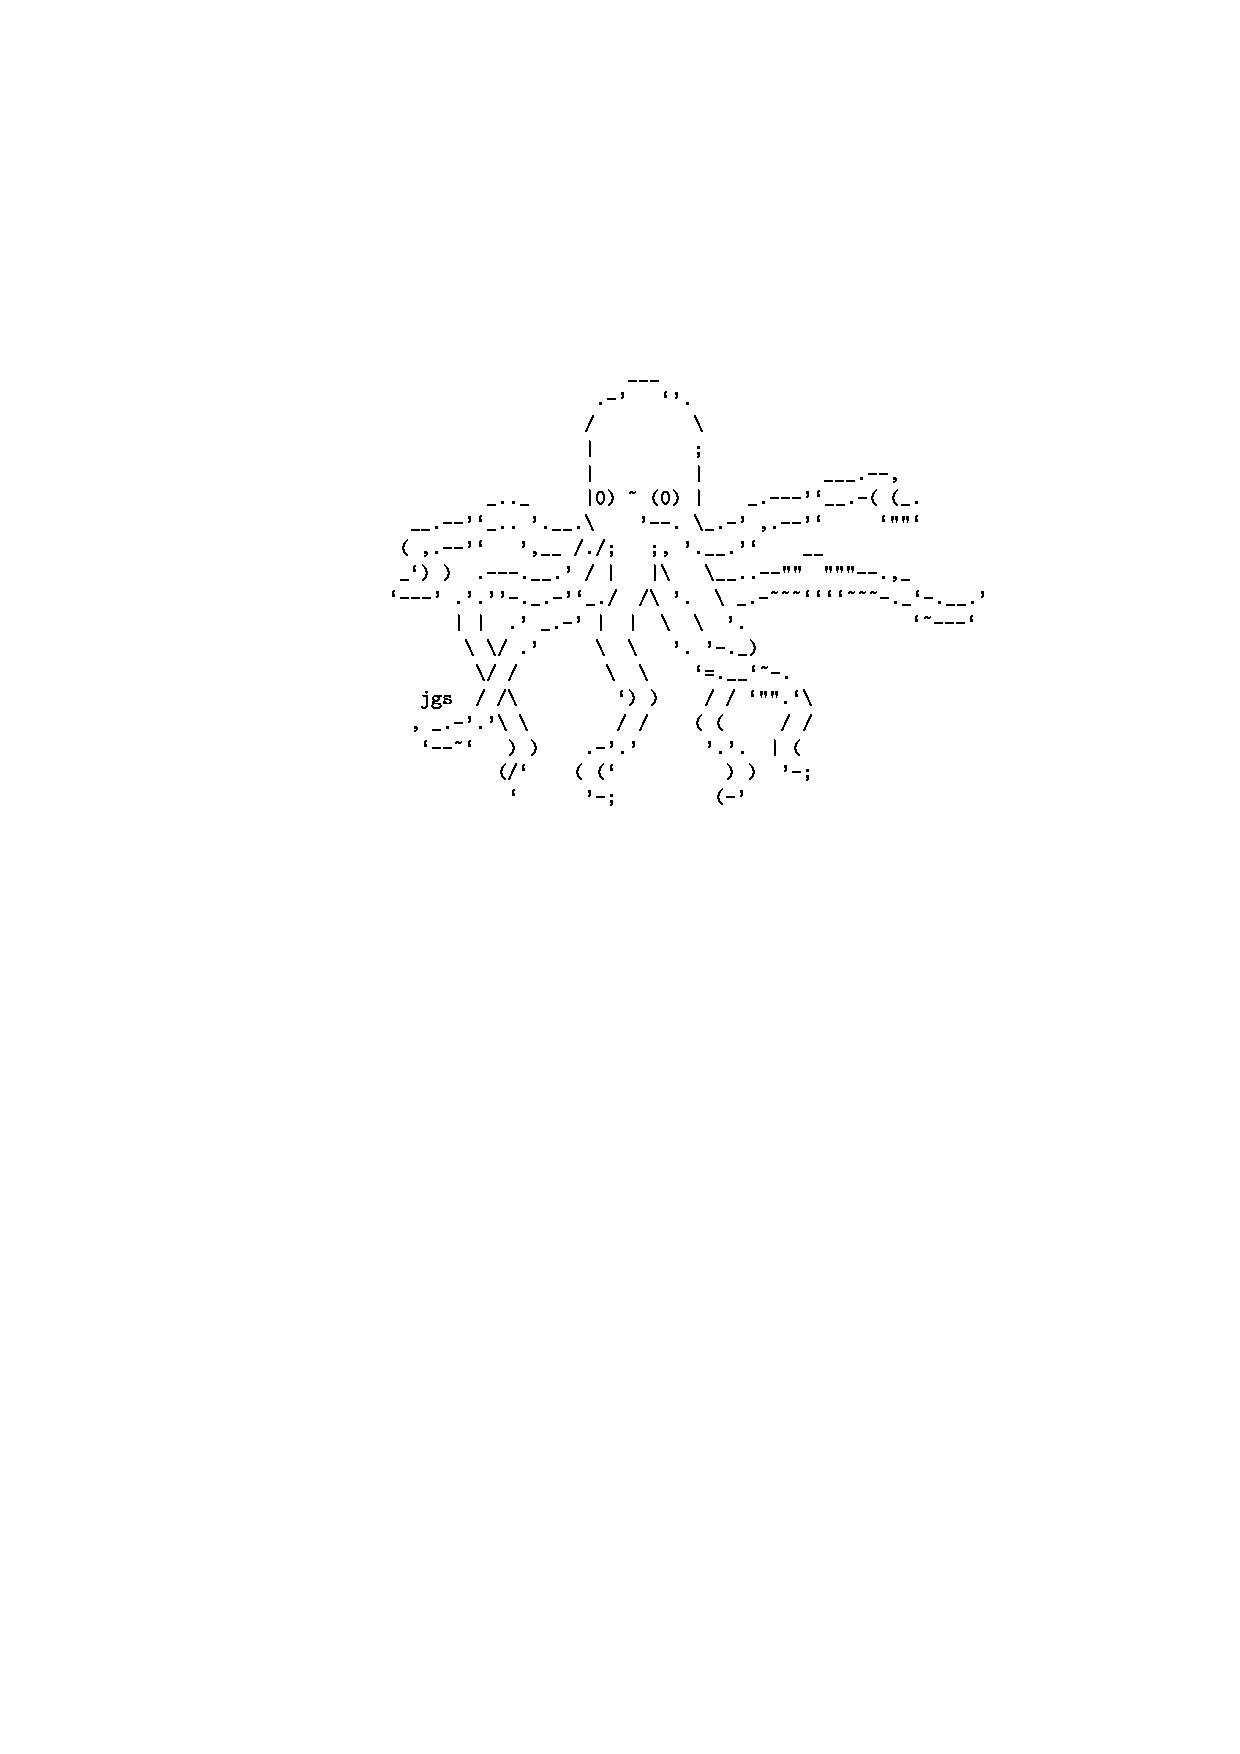
\includegraphics[height=5cm]{img/cover}
\end{flushright}

\vspace{-2cm}

\begin{flushleft}
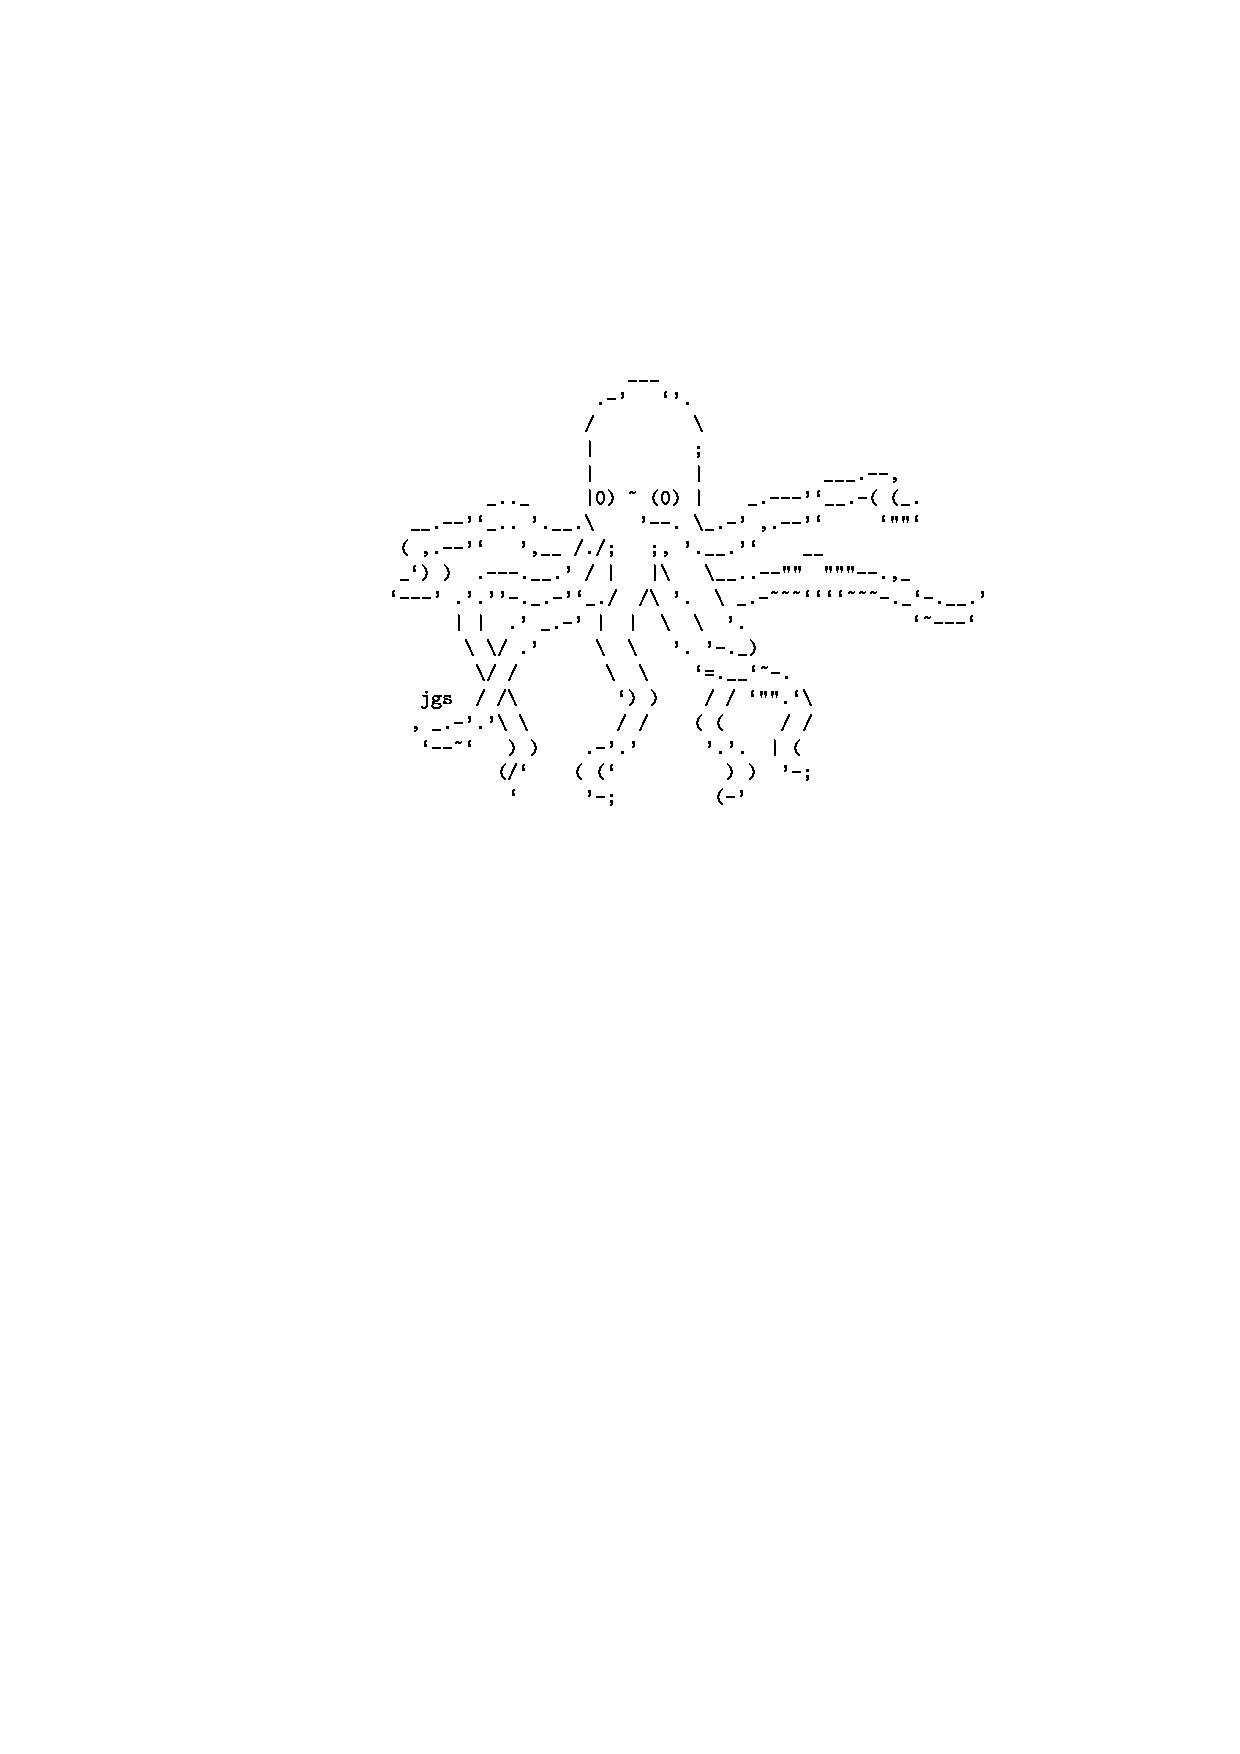
\includegraphics[height=5cm]{img/cover}
\end{flushleft}

\begin{flushright}
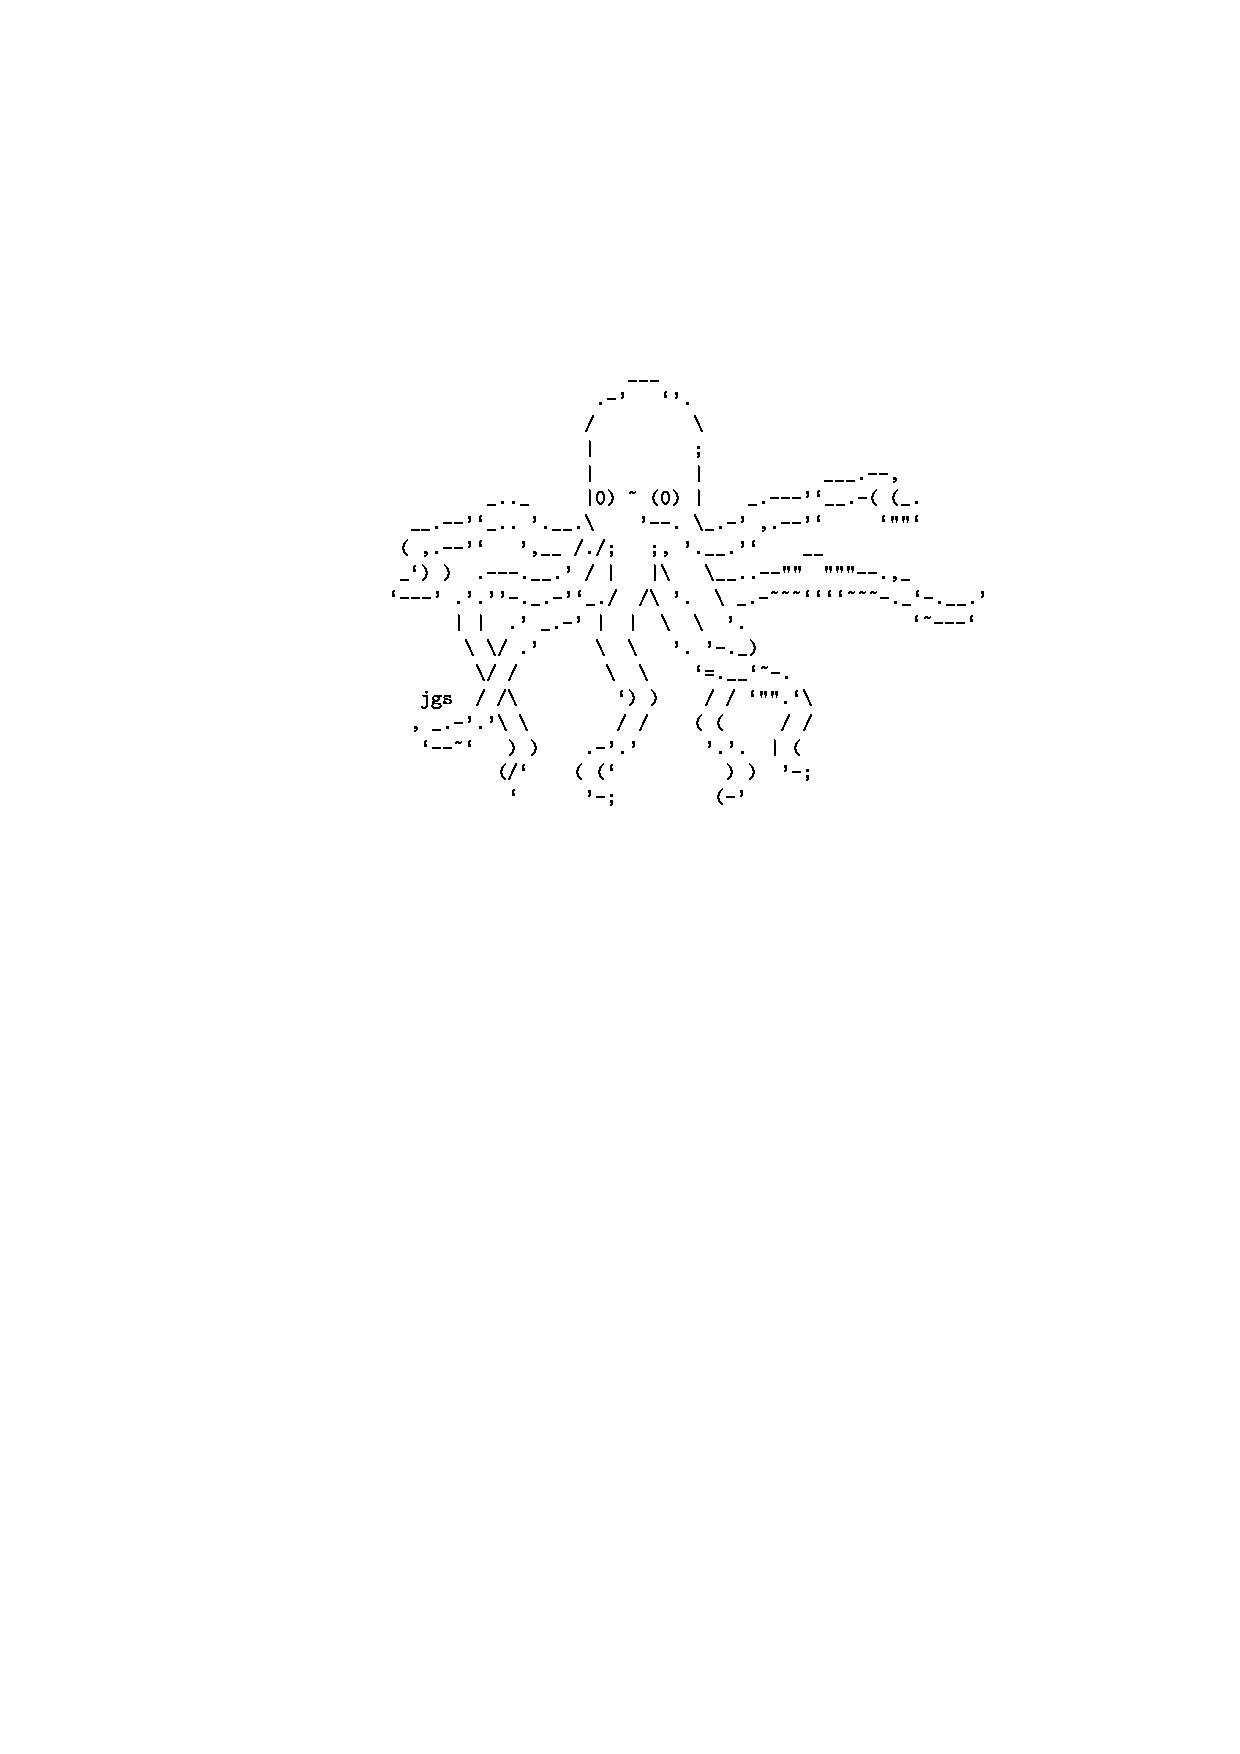
\includegraphics[height=5cm]{img/cover}
\hspace*{2cm}
\end{flushright}


\thispagestyle{empty}

\pagebreak

\tableofcontents

\pagebreak

\section{General remarks}

This tutorial should make your start with OCTOPUS a little easier. It is based
on a hands-on class given in Berlin. The tutorial will provide you with a
couple of examples of different things that you can do with OCTOPUS. It is by
no means complete, there are a lot of other things that OCTOPUS can do for you,
but hopefully it gives you an idea of how to use the different options. You can
find more information in the online manuel at \tt
http://www.tddft.org/programs/octopus. \rm

OCTOPUS is a real-space code that works with equally spaced grids. The spacing
can be different in different directions. All quantities are given in atomic
units unless stated otherwise. It also treats all numbers internally as double
precision but you as the user don't have to worry about that.

\section{The harmonic oscillator in 1D} 

As the first example we use the standard textbook harmonic oscillator in one
dimension and fill it with two non-interacting electrons. Now we just have to
tell OCTOPUS that we want to do exactly that. The program expects you to write
an input file called {\bf inp}, where all the initial information is stored.
OCTOPUS will always look for this file in the directory you are working in. So
we suggest you just make a subdirectory for every example in this tutorial and
then you can always give the input file the same name.

OCTOPUS already knows a couple of things that make the input a lot easier. Most
of the usual functions like \tt sin \rm and \tt cos \rm but also \tt sqrt \rm
and many more are known. OCTOPUS also knows the coordinates \tt x, y, z, r \rm
that you will need to put in potentials. It is also capable of working with
pseudopotentials, as we will see later on. Some parts of the input are expected to
be given as strings and have to be written in quotation marks.

So now it's time to write the first input file. So get your favourite text
editor, write the following lines and save the file as {\bf inp}.

\begin{verbatim}
SystemName="HO" 
CalculationMode = 1
Dimensions=1 
NonInteractingElectrons = yes
radius = 10
spacing = 0.1
% Species 
"HO"|1|2|"0.5*x^2" 
%
% Coordinates
"HO"|0|0|0|no
%
\end{verbatim}

Most of the entries are kind of self-explaining. In the first line, we simply
assign a meaningfull name to the system. That's just for us to remember what
this input file was for. The CalculationMode 1 is a static  calculation, so
OCTOPUS will simply minimize the energy for whatever geometry you give it. If
you assign the correct geometry it will therefore calculate the ground-state
energy. Since we stated the correct geometry for our problem (since we deal
with only one harmonic oscialltor there is nothing you can do wrong) we will
get the ground-state energy of the harmonic oscillator. We will come back to
this geometry argument once we have more atoms. We chose the electrons to be
non-interacting. The next two entries specify a radial grid with radius 10 and
spacing 0.1. These values have to be chosen such that the calculation
converges. We will see in a later example how they can change the results. Now
we define Species, which is nothing else than the atoms or elements fo the
system we want to calculate. In our case it is a harmonic oscillator, so we
give the default name ``HO'', the second entry corresponds to its mass that we
choose to be one. The next entry is the number of valence electrons, in our
case 2. Finally, the last entry is the potential that resembles this kind of atom, so
just the harmonic oscillator potential. Note that the potential and the name
have to be given as strings. Since Species are defined in a block, this part
starts with a \tt \% \rm and also ends with a \tt\%\rm. The next block  fixes
the coordinates. We simply put one harmonic oscillator at the origin and don't
allow it to move, that is what the \tt no \rm stands for.

Now one can execute this file by the command

\tt octopus
\rm

OCTOPUS will then calculate the ground-state energy and occupation numbers for
the given geometry and finds an energy of 0.5 and an occupation number of 2,
just as we expect from basic quantum mechanics. Apart from this OCTOPUS will
also produce a file called {\bf out.oct}. This file is a plain-text file that
contains the information OCTOPUS reads from your input file. If you look at it,
you will find the information you included in your file and additional entries
which have a \tt \#default \rm comment to it. So things you did not specify in
your input file will be assigned their default values. You can also use this
file to find out what options you can specify and what the appropriate variable
is called. So it's a good idea to have a look at this file from time to time.
When  OCTOPUS had a successfull run it will also create a subdirectory called
{\bf static} where it will store all its output. From the previous calculation
you will find a file called {\bf info} in that directory. It is also a plain
text file so just have a look at it. It will give you detailed information about
the mesh OCTOPUS used and the results with errors and convergence criteria and
so on. In CalculationMode=1 the convergence criteria is the density.

Now we can play a little bit with the input file and add some other features.
For example we could think of not only calculating the ground-state but also
some excited states. This can be done by changing the CalculationMode to 3

\begin{verbatim}
CalculationMode=3
\end{verbatim}

in the input file. In this mode OCTOPUS will not only give you the ground state
but also five excited states. This is just a default value that you can change
yourself by putting an extra line

\begin{verbatim}
UnoccNumberStates=10
\end{verbatim}

that will calculate 10 excited states. A thing to note here is that OCTOPUS
will need the density for this calculation. (Actually for non-interacting
electrons the density is not needed for anything, but since OCTOPUS is designed
for interacting electrons it will try to read the density anyways.) So if you
have already performed a static calculation (CalculationMode=1) it
will just use this result. If you have not done this calculation OCTOPUS will
do that first. Compared to the ground-state calculation we also have to change
the convergency criterium. The unoccupied states do not contribute to the
density so they might not (and actually will not) converge properly if we use
the density for the convergence check. Therefore, OCTOPUS now checks whether all
calculated states converge seperately by just looking at the biggest error in
the wave-functions. From the calculation you get another file in the {\bf
static} directory called eigenvalues. The info-file will only contain the
information about the ground-state, all eigenvalues and occupation numbers will
be in the eigenvalues-file.

If we also want to plot, say the wave-function, at the end of the calculation,
we have to tell OCTOPUS to give us this wave-function and how it should do this.
We just include

\begin{verbatim}
OutputWfs=yes
OutputAxisX=yes
\end{verbatim}

The first line tells OCTOPUS to give out the wave-functions and the second line
says it should do so along the x-axis.

We can also select the wave-functions we would like as output, for example the
first and second, the fourth and the sixth. (If you don't specify anything
OCTOPUS will give them all.)

\begin{verbatim}
OutputWfsNumber="1-2,4,6"
\end{verbatim}

OCTOPUS will store the wave-functions in the same folder {\bf static} where the
info file is, under a meaningfull name. They are stored as pairs of the x
coordinate and the value of the wave-function at that position x. One can
easily plot them with gnuplot or a similar program.

It is also possible to extract a couple of other things from OCTOPUS like the
density or the Kohn-Sham potential. We will get to some of them in the following
examples.

\section{Helium atom in 1D}

The next example will be the Helium atom in one dimension which also has two
electrons just as we used for the harmonic oscillator. Instead of describing two
electrons in one dimension we will describe one electron in two dimensions. From
the potential 

\begin{equation}
\frac{-2}{\sqrt{1+x^2}}+\frac{-2}{\sqrt{1+y^2}}+\frac{1}{\sqrt{1+(x-y)^2}}
\end{equation}

one can see that this makes absolutely no difference. Whether we regard $x$ and
$y$ as the coordinates of two different particles in one dimension or as the
coordinates of the same particle along the two axes in two dimensions is
entirely up to us. Since it is usually easier to treat only one particle, we
will solve the one-dimensional Helium atom in two dimensions.
We will also get a two dimensional wave-function. In order to plot this
wave-function we specify an output plane instead of an axis. With the different
potential and one more dimension the new input file looks the following

\begin{verbatim}
SystemName="He"
CalculationMode=1
Dimensions=2
NonInteractingElectrons=yes
radius=10
spacing=0.1
OutputWfs=yes
OutoutPlaneZ=yes
#OutputWfsNumber="1-2,4,6"
%Species
"He"|4|1|"-2/(1+x^2)^(1/2)-2/(1+y^2)^(1/2)+1/(1+(x-y)^2)^(1/2)"
%
%Coordinates
"He"|0|0|0|no
%
\end{verbatim}

We have also commented out the line that chooses the wave-functions for the
output. (OCTOPUS will always ignore anything that comes after a \tt \#\rm.)
Since we went back to CalculationMode=1 only the ground-state is calculated. 

The calculation will take longer than the one for the harmonic oscillator and
should converge within 16 iterations. If it happens that you want to stop the
calculation and then restart it there is good news, OCTOPUS allows you to do
this. You might have noticed that apart from the {\bf static} directory there is
also a {\bf tmp} directory in your working directory. If you go there you will
find a restart.static file. This is a binary file and it is not platform
independent (so don't transfer it from a PC to an Alpha). OCTOPUS stores all the
information it needs to continue the calculation in that file. You can use this
information by simply changing the CalculationMode to 2

\begin{verbatim}
CalculationMode=2
\end{verbatim}

If you do this in the helium input file that we just used and rerun OCTOPUS the
calculation will converge with just one iteration, because you use the already
converged data from restart.static.

Now you can do just the same we did for the harmonic oscillator and change the
CalculationMode to three and calculate five unoccupied states. This will take
some time (like 188 iterations), so if you feel hungry or need to read your
email, this is the time to eat something or start pine. 

Apart from the eigenvalues and occupation numbers we asked OCTOPUS to put out
the wave-functions. There is a side-remark here that has nothing to do with the
program itself put with basic quantum mechanics. There are degenerate
eigenvalues in the helium atom (in the calculation the 4th and 5th eigenvalue
should come out quite similar). This means that you have two or more
wave-functions for the same energy. Also any linear combination of these
wave-functions will be an eigenfunction for the same energy. The correct
wave-functions can be chosen by symmetry considerations. Since OCTOPUS does not
have the ability to choose, the given wave-functions might look very funny.
This remark is not only valid for helium but for any system that has degenerate
eigenvalues.

\section{Benzene}

So now comes the first real system. We will work in three dimensions and also
make the electrons interacting. So you can just comment the line with the
NonInteractingElectrons out. We will also change the unit system to electron
volts and~\AA since the coordinates for benzene will be given in
Angstr\"om. You can either put them in by hand just as we did before, but you
can also ask OCTOPUS to read the coordinates from a file by the following comand

\begin{verbatim}
XYZCoordinates="benzene.xyz"
\end{verbatim}

provided you have a file called benzene.xyz in the directory. This will replace
the whole Coordinates block that we had before. There are certain
requirements that OCTOPUS has concerning coordinate files. The benzene.xyz
should looks the following (including empty lines!!!)

\begin{verbatim}
12

 C  0.000  1.396  0.000
 C  1.209  0.698  0.000
 C  1.209 -0.698  0.000
 C  0.000 -1.396  0.000
 C -1.209 -0.698  0.000
 C -1.209  0.698  0.000
 H  0.000  2.479  0.000
 H  2.147  1.240  0.000
 H  2.147 -1.240  0.000
 H  0.000 -2.479  0.000
 H -2.147 -1.240  0.000
 H -2.147  1.240  0.000
\end{verbatim}

The first line specifies the total number of atoms that are given in the file.
The second line is a comment line, if you don't have comments, leave it blank
but do not erase the line. All following lines give the coordinates of the atoms
with the normal \tt x, y, z \rm order of the different directions in space. All
the numbers up there are in \AA so we have to change the units in OCTOPUS
to electron volts and \AA as well. We do so by adding a line

\begin{verbatim}
Units="eVA"
\end{verbatim}

In three dimensions there are several geometries that require a radius as one
variable. So the specification of the radius is no longer sufficient to fix the
geometry we are working with. We therefore have to specify the BoxShape which
we will choose to be a sphere. Since we are working in three dimensions by now
we have to think a little more carefully about the mesh we are using. If you
have a look at benzene coordinates you will see that the biggest coordinates
are around 2.1. So there is no need to extend the mesh all the way to 10, 5
should be enough. We also made the spacing a little larger. (The calculation
will still take long enough.) You can play a little bit with these values and
see if the results converge. We specified one more thing in this input file and
that is the OutputDX. OCTOPUS will therefore give all its output in a form that
you can read with Open DX. 

\begin{verbatim}
SystemName="Benzene"
CalculationMode=1
Units="eVA"
Dimensions=3
#NonInteractingElectrons = yes
BoxShape=sphere
radius=5
spacing=0.15
OutputWfs=yes
OutputDX=yes
%Species
"H"|1.0079|1|"tm2"|0|0
"C"|12.011|6|"tm2"|1|1
%
XYZCoordinates="benzene.xyz"
\end{verbatim}

The definition of the species looks different from the previous examples. Since
we are working with interacting electrons we better use pseudopotentials to
describe them. We therefore tell OCTOPUS that we want to describe the hydrogen
and carbon atoms with a Troullier-Martinez type pseudopotential. The two last
numbers then specify the highest angular momentum and the momentum that is used
as a local potential. (You can get these pseudopotentials from \tt
http://www.tddft.org/programs/octopus and just click on pseudopotentials\rm.)
Save them in files called H.ascii and C.ascii in your directory. OCTOPUS will
look for these files and then just use them.


\section{Methane}

For the methane molecule we will use the very same pseudopotentials that we used
for benzene already. In this example we will play a little bit with the spacing
and the dimensions of the mesh as well as the bonding length of the CH bond.

In the input file we define a variable CH that represents the bond length
between the carbon and the hydrogen atoms. From our basic chemistry class we
know that methane has a tetrahedral structure. If we put the carbon atom at the
origin the hydrogen atoms have the coordinates given in the following input
file.

\begin{verbatim}
SystemName="CH4"
CalculationMode=1
Units="eVA"
radius=3.5
spacing=0.25
CH=1.2
%Species
"C"|12.011|6|"tm2"|1|1
"H"|1.0079|1|"tm2"|0|0
%
%Coordinates
"C"|0|0|0|no
"H"|CH/sqrt(3)|CH/sqrt(3)|CH/sqrt(3)|no
"H"|-CH/sqrt(3)|-CH/sqrt(3)|CH/sqrt(3)|no
"H"|CH/sqrt(3)|-CH/sqrt(3)|-CH/sqrt(3)|no
"H"|-CH/sqrt(3)|CH/sqrt(3)|-CH/sqrt(3)|no
%
\end{verbatim}

We start with a bond length of 1.2~\AA but that's not so important at the
moment since we will optimize this number. (You should not use 5 or so, but
something slightly bigger than 1~\AA is fine.) If you use the given input
file you should find the following values in the resulting info file

\begin{verbatim}
Eigenvalues [eV]
   #   Eigenvalue    Occupation      Error (1)
   1   -15.505477       2.000000      (1.9E-06)
   2    -9.008944       2.000000      (3.3E-06)
   3    -9.008944       2.000000      (3.3E-06)
   4    -9.008944       2.000000      (3.3E-06)

Energy:
      Ion-ion     =    236.08676335
      Eigenvalues =    -85.06461671
      Potentials  =   -288.75407490
      Exchange    =    -69.86363967
      Correlation =    -11.02145481
      Total       =   -218.61702274
\end{verbatim}

Now the question is, are these values converged or not. This will depend on the
spacing and the radius. The only way to answer this question is to try other
values for the radius and the spacing. We will start with the spacing. Since we
are interested in the total energy of the system, we will look at the changes of
its value. We will keep all entries in the input file fixed except for the
spacing that we will make smaller by 0.025 all the way down to 0.1. So you have
to run OCTOPUS several times to get the following results

\begin{verbatim}
0.25           -218.61702274
0.225          -218.67897072
0.2            -218.33197586
0.175          -218.05746540
0.15           -218.02394141
0.125          -218.00237716
0.1            -217.99662781
\end{verbatim}

If you give these numbers to gnuplot you will get a curve like this

\begin{figure}[h]
\begin{center}
\includegraphics[width=7cm,angle=-90]{img/spacing}
\end{center}
\caption{The dependence of the total energy on the spacing}
\end{figure}

As you can see from this picture, the total energy is converged to within 0.1~eV
for a spacing of 0.175. So we will use this spacing for the next calculations
and play with the radius of the box. We will change make the radius bigger in
steps of 0.5. Doing this we get

\begin{verbatim}
3.5             -218.05746540
4.0             -218.14891908
4.5             -218.16777476
\end{verbatim}

If we again ask for a convergence up to 0.1~eV we should use a radius of 4.0
Angstr\"om. 

Now that we have fixed the two parameters we can procede and optimize the bond
length. This time we don't have to do this by hand, we let OCTOPUS do the work
for us. We simply have to allow the atoms to move, so we change all these ``no''
that we have there to ``yes''. We also have to change the CalculationMode to 10
which is geometry optimization and we have to specify a condition for the
calculation to stop. OCTOPUS calculates the forces on each atom in this
calculation mode and we can use these forces by allowing for a tolerance of for
example 0.01 (what units?). We should also tell OCTOPUS to give us the result of
the calculation. So we have to specify the following things in the input file

\begin{verbatim}
SystemName="CH4"
CalculationMode=10
Units="eVA"
radius=4.0
spacing=0.175
GOTolerance=0.01
OutputGeometry=yes
OutputDX=yes
OutputELF=yes
%Species
"C"|12.011|6|"tm2"|1|1
"H"|1.0079|1|"tm2"|0|0
%
CH=1.2
%Coordinates
"C"|0|0|0|yes
"H"|CH/sqrt(3)|CH/sqrt(3)|CH/sqrt(3)|yes
"H"|-CH/sqrt(3)|-CH/sqrt(3)|CH/sqrt(3)|yes
"H"|CH/sqrt(3)|-CH/sqrt(3)|-CH/sqrt(3)|yes
"H"|-CH/sqrt(3)|CH/sqrt(3)|-CH/sqrt(3)|yes
%
\end{verbatim}

OCTOPUS will give you a file in the static folder that is called geometry.xyz.
I this file it writes the coordinates of all the atoms that result from the
calculation. If you calculate the CH bond length from these coordinates you
should find something like 1.0959~\AA. So you should change the bond
length in you input file to that value for the following calculations. We also
asked OCTOPUS to give us the ELF for the methane molecule in a format that can
be read by Open DX. So just have a look at it. 

Finally, we want to calculate the spectrum of the methane molecule. We will use
a time-dependent calculation and therefore change to CalculationMode=5. We will
have to specify some other parameters for this, but before we go into details a
few more remarks on the general idea of the calculation.

We will excite the molecule with a small electric field. It has to be small
since a spectrum is a linear response effect and linear response is only valid
for small fields. We definitely don't want to ionize the molecule for example.
Since we do not know which frequencies methane can absorb (that's in fact what
we want to calculate), we will just use all frequencies. This sounds funny from
the experimental point of few but there is no problem doing this on a computer.
We will use an electric field of the form

\begin{equation}
E(t)=E\delta(t-t_0)
\end{equation}

with a small amplitude $E$. In order to keep this simple we will choose $t_0=0$.
If we do a Fourier transform of this electric field we will see that all
frequencies appear in the transformed electric field $E(\omega)$. With this
electric field we will kick the methane molecule a little bit (since $E$ is
small) at time $t_0=0$ and then just let it evolve. What will happen is that
most frequencies will die off exponentially and only the eigenfrequencies of the
system will survive. We therefore just have to wait and get the spectrum of the
methane molecule.


\appendix

\section{Calculation Modes}

\begin{tabular}{rl}
1 & start static calcualtion\\
2 & resume static calculation\\
3 & start calculation including unoccupied states\\
4 & resume calculation of unoccupied states\\
5 & start time-dependent calculation\\
6 & resume time-dependent calculation\\
7 & start calculation of static polarizability\\
8 & resume calculation of static polarizability\\
9 & missing\\
10 & optimization of geometry\\
11 & calculation of the phonon spectrum\\
12 & optimum control mode (is this already working?)\\
99 & printing an octopus recipe
\end{tabular}
\end{document}
